 % For pdflatex in arxiv
%\pdfoutput=1

% Set the document class to a generic article
\documentclass{article}

% Import helpful packages
\usepackage{amsmath}
\usepackage{amsfonts}
\usepackage{amssymb}

% Use Natbib for handling the bibliography
\usepackage[round,
				    authoryear,
				    colon]{natbib}
\bibliographystyle{plainnat}

% For accents over letters
%\usepackage[utf8]{inputenc}
\usepackage[T1]{fontenc}

% For highlighting
\usepackage{color, soul}

% For handling of urls in bibtex file
\usepackage{url}
\def\UrlBreaks{\do\/\do-}    % use to break urls at hyphens

% Configure page margins
\usepackage[margin=1in]{geometry}

% For handling images
\usepackage{graphicx}

% For making tables pretty
\usepackage{booktabs}
\usepackage{caption}

% Declare article info
\title{Some Title}
\author{All of us}


% Body of document
\begin{document}

\maketitle

% Add sections
\section*{Abstract}

In this chapter, we focus on using causal graphs to make causal inferences in choice modelling contexts.
We address a longstanding disconnect whereby choice modellers have not adopted techniques from causal inference researchers, even when trying to make causal inferences.
To bridge this disconnect, we conduct simulation studies to first demonstrate the need for paying close attention to causal graphs in choice modelling.
We then present new guidelines, methods, and perspectives for the construction and validation of causal graphs, complete with empirical examples.
Next we give examples and direction for using one's causal graphs to make causal inferences in common choice modelling scenarios, including those with latent confounding.
Finally, throughout the chapter, we point readers to more information through extensive literature reviews.
At the chapter's conclusion, choice modellers should have a much clearer understanding of (or references to find out about) why they should use causal graphs, what graphs to use for their dataset, and how they can use a given causal graph to complete their causal inferences.


\section{Introduction}
\label{sec:intro}

The following chapter is concerned with the existing disconnect between the 
fields of travel demand modeling and causal inference. 
More specifically, the chapter is motivated by the current lack of use of methods and findings from 
the causal inference literature in travel demand modeling. 

More often than not, the development of behavioral models in transportation, 
specifically transportation demand models, is driven by the need to evaluate 
the impact of external interventions, in the form of alternative policies, on a 
certain outcome of interest. 
These questions that transportation demand models 
are built to answer are causal by definition: we are interested in how the 
system reacts to \textit{external} interventions. 
Yet, when those models are 
developed, there is very little consideration given to causality, and when 
causal concepts are accounted for, the process is done implicitly without a 
formal framework. 

While the field of transportation demand modeling could benefit greatly from 
incorporating causal inference techniques, there are barriers that have made 
this integration slower than what one would hope. 
These barriers stem from the difference between the types of problems transportation demand modelers deal with and those that are typically studied in the causal inference literature. 
Perhaps the main fundemental difference is that demand modelers 
are typically trying to forecast the impacts of policies that haven't been 
implemented or seen before, which requires additional work and a change to the
typical causal modeling workflow in order to translate a given policy 
(treatment) into a set of characteristics and variables that exist in the
data and system at hand (please refer to \citet{brathwaite_2018_causal} for a 
more thorough discussion of those barriers). 
While those barriers make the problem of demand modelers harder, there is still a lot to gain from 
incorporating causal inference techniques where appropriate, and to contribute
in turn where the literature lacks.  

The relevance of this topic now is motivated by the significant boost in the causal inference literature recently, both in the potential outcomes and the causal graphical modeling frameworks.
The goal of this chapter is to formalize a workflow for approaching 
transportation demand modeling problems from a causal perspective. 
We will draw heavily on the use of directed acyclic graphs (DAGs) formalized by \citet{pearl_causality_2000} as a means of representing the modeler's knowledge and assumptions about a given problem. 
The chapter will provide an overview of DAGs, the 
testable implications that come with one's causal representation, the main 
tests that one could do to falsify or justify a given causal graph, and then how 
to use a causal graph to estimate the causal relationships of interest. 
We will demonstrate the use of this framework through simulations, where we 
clearly show the benefits and implications of this approach as opposed to 
traditional approaches. 
The last part of this chapter deals with the more complicated issue of latent 
confounding, where one variable confounds two or more variables in the causal 
graph. This type of confounding creates variations in the outcome variable that are not caused by 
the confounded variables but are correlated with it, which biases the estimated 
causal effects of those variables if nothing is done to account for the 
confounding. 
We focus on a recent technique to deal with latent confounding suggested by \citet{wang_2019_blessings} to address unobserved confounding when collecting additional data is not feasible. 
We describe this problem in more details in section 7.


\section{Perils of disregard}
\label{sec:graph-importance}

As stated in Section \ref{sec:intro}, transportation demand models are used to evaluate the impact of policies on a certain
transportation demand related outcome. As an example, consider the proposals from the following fictitious scenarios:
\begin{itemize}
 \item Based on input from the public, the Department of Transportation (DOT) is considering implementing a new parking policy.
 This proposed policy would change prices and restrict availability to discourage individuals from parking in the central business district.
 The DOT and its constituents believe that this policy will encourage people to use more active transportation modes (e.g., walking, biking, etc.) and cause them to drive less.
 \item A certain DOT is considering constructing a streetcar (trolley, tram) line in a low/mid-income area in its jurisdiction.
 Citing examples from other cities and countries, the DOT claims that the new streetcar line will create more transit oriented developments and increase economic activity in the areas surrounding the proposed project.
 \end{itemize}

%% TODO: Present an example or two of real life project proposals?

Thinking more closely about these proposals, it is clear that they assume a causal relationship between the proposed project/policy and the desired goals.
The DOT in question analyzed data, concluding that such a policy or project would cause the desired output and achieve the desired goal.
In the presented scenarios, the DOT claims that implementing the new parking policy will cause an increase the share of
active transportation modes in the central business district and that constructing the proposed streetcar line will
cause more transit oriented developments and economic activity.

Policymakers base their analyses and conclusions on hypotheses or beliefs of how the world operates.
In other words, the data analysis is based on specific beliefs about the data generating process.
However, policymakers often do not present these beliefs in a clear and concise manner.
As a result, these proposals maintain an obscure representation of how the policy or project will achieve their desired goals.

DAGs allow one to clearly encode their assumptions about the data generating process and the problem at hand.
Researchers and practitioners have made use of DAGs in fields ranging from medicine and epidemiology (\citet{shrier_2008_reducing, sung_2012_reducing}) to economics (\citet{white_2011_covariate}) and have found them to be practical.

Likewise, DAGs could prove useful in addressing transportation policy questions.
\citet{brathwaite_2018_causal} have proposed a framework illustrating how practitioners and researchers can use DAGs to answer such transportation modelling questions in a causal context.
However, \citet{brathwaite_2018_causal} did not show an empirical application of their framework and how it results in different conclusions when compared to traditional modelling approaches.

In this section, we will present an example illustrating the importance of using DAGs in transportation demand modelling.
Specifically, we will illustrate how different assumptions about the data generating process result in different conclusions, even while assuming the same outcome model.
To make our point, we build upon \citet{brathwaite_2018_causal}.
Here, we present an empirical exercise using a simplified transportation modelling problem.
Before going any further, we note that this example is illustrative, and it does not reflect all complexities in a typical transportation choice modelling problem.
Indeed, it is not our primary goal in this section to recover the causal effect of the proposed intervention.
Instead, we are most interested in showing how different DAGs would result in different conclusions about the effect of the proposed intervention.

Let us assume that a company wants to reduce its workforce carbon footprint by moving its employees closer to their campus.
We would like to forecast how such an intervention would change the share of employees driving to work.
We model this travel mode choice problem based on a dataset from \citet{brathwaite_asymmetric}.
This dataset is based on the 2012 California Household Travel Survey, and it
contains approximately 4000 home-based school or work tours made by approximately 3850 individuals in the California Bay area.
The dataset includes eight travel modes. 
For our illustrative purposes, we focus on the following car-centric modes:

\begin{itemize}
   \item Drive Alone: The individual uses a private vehicle to make the trip
   \item Shared Ride 2: The individual shares an automobile ride with one more individual
   \item Shared Ride 3+: The individual shares an automobile ride with two or more individuals
\end{itemize}

Readers interested in a more detailed description of the dataset can refer to \citet{brathwaite_asymmetric}.
For the purposes of this exercise, we treat the multinomial logit model (MNL) defined in \citet{brathwaite_asymmetric} as the true outcome generating model.

In this model, the systematic utility equations of the car-centric modes defined above are specified as follows:
\begin{equation*}
   \begin{aligned}
   \textrm{Utility} \left(\textrm{Drive Alone}\right) &= \beta_{\textrm{travel\_time}} \times \textrm{Travel\_Time} + \beta_{\textrm{cost\_per\_distance\_drive\_alone}} \times \textrm{Cost\_per\_Distance}_{\textrm{da}} \\
   &\quad + \beta_{\textrm{autos}} \times \textrm{Number\_of\_Autos} \\
   \textrm{Utility} \left(\textrm{Shared Ride 2}\right) &= ASC_{\textrm{shared\_ride\_2}} + \beta_{\textrm{time\_drive}} \times \textrm{Travel\_Time} \\
   &\quad + \beta_{\textrm{cost\_per\_distance\_shared\_ride\_2}} \times \textrm{Cost\_per\_Distance}_{ \textrm{sr2} } + \beta_{\textrm{autos}}  \times \textrm{Number\_of\_Autos} \\
   &\quad + \beta_{\textrm{cross\_bay}} \times \textrm{Cross\_Bay} + \beta_{\textrm{hh\_size}} \times \textrm{Household\_Size} \\
   &\quad + \beta_{\textrm{n\_kids\_hh}} \times \textrm{Number\_of\_kids} \\
   \textrm{Utility} \left(\textrm{Shared Ride 3+}\right) &= ASC_{\textrm{sr3+}} + \beta_{\textrm{time\_drive}} \times \textrm{Travel\_Time} \\
   &\quad + \beta_{\textrm{cost\_per\_distance\_sr3+}} \times \textrm{Cost\_per\_Distance}_{\textrm{sr3+}} + \beta_{\textrm{autos}}  \times \textrm{Number\_of\_Autos} \\
   &\quad + \beta_{\textrm{cross\_bay}} \times \textrm{Cross\_Bay} + \beta_{\textrm{hh\_size}} \times \textrm{Household\_Size} \\
   &\quad + \beta_{\textrm{n\_kids\_hh}} \times \textrm{Number\_of\_kids} \\
   \end{aligned}
\end{equation*}

Note that, since we consider this model to be the true outcome model, there are no latent variables we need to account for.
Below is a description of the key variables included in the model:

\begin{itemize}
  \item Total Travel Distance: the total travel distance for individual i and mode j, for all available modes for individual i during trip t of tour l.
  \item Total Travel Cost: the travel cost in dollars for individual i and mode j, for all available modes for individual i during trip t of tour l.
  \item Total travel time: the travel time in minutes for individual i and mode j, for all available modes for individual i during trip t tour l.
  \item Number of Autos: the number of automobiles owned by individual i's household.
  \item Number of Licensed Drivers: is the number of licensed drives in individual i's household.
  \item Number of Kids: the number of kids in individual i's household.
  \item Cross-bay trip: a binary variable indicating whether the trip t in tour l for individual i is a cross-bay trip.
\end{itemize}

Figure \ref{fig:IND_GRAPH} illustrates the DAG where all explanatory variables in each utility equation are marginally independent.
This DAG is equivalent to what an analyst assumes when they only update the variables directly impacted by a given policy, without considering the dependencies between the explanatory variables. 
To illustrate the problem with this approach, consider the case where the ``true'' data generating process that reflects the dependencies between the covariates is as shown in Figures \ref{fig:DA_causal_2} through \ref{fig:SR3_causal_2}. 
Under this generative model, intervening on one variable would also result in changes to other variables that are dependent on it.
The goal of our simulation exercise is to show that ignoring the true generative model of the data can result in arbitrarily biased treatment effects, even if the analyst knows the true outcome model.

\begin{figure}
   \centering
   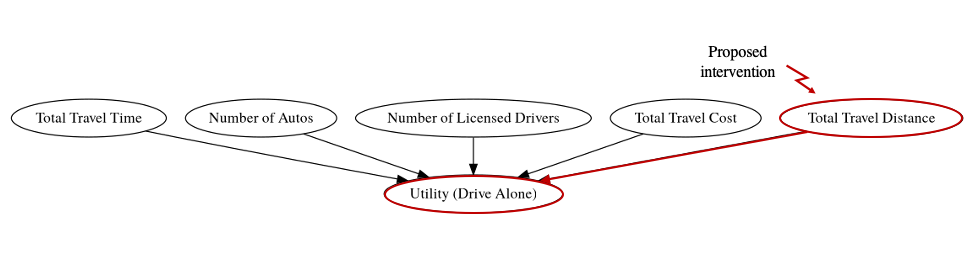
\includegraphics[width=0.75\textwidth]{Independent_graph}
   \caption{Causal Graph with Independent Covariates}
   \label{fig:IND_GRAPH}
\end{figure}

\begin{figure}
   \centering
   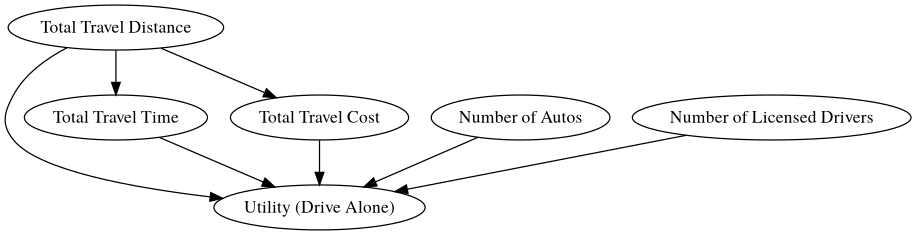
\includegraphics[width=0.75\textwidth]{DA_interacting_graph}
   \caption{Causal Graph for the Drive Alone Utility Function}
   \label{fig:DA_causal_2}
\end{figure}

\begin{figure}
   \centering
   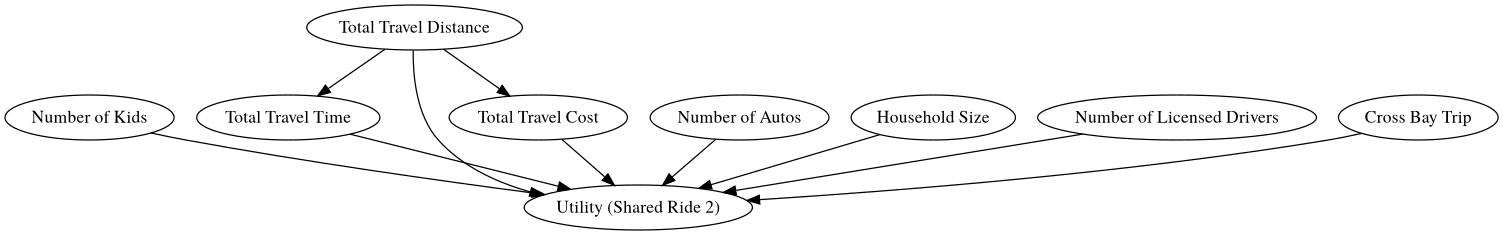
\includegraphics[width=0.75\textwidth]{SR2_interacting_graph}
   \caption{Causal Graph for the Shared Ride 2 Utility Function}
   \label{fig:SR2_causal_2}
\end{figure}

\begin{figure}
   \centering
   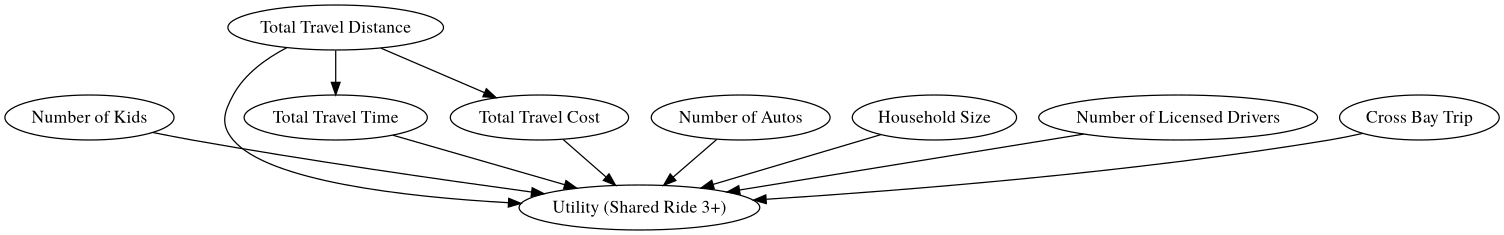
\includegraphics[width=0.75\textwidth]{SR3_interacting_graph}
   \caption{Causal Graph for the Shared Ride 3+ Utility Function}
   \label{fig:SR3_causal_2}
\end{figure}

Using the same outcome model, we:
\begin{itemize}
   \item Simulate data from the DAGs shown in Figure \ref{fig:IND_GRAPH} through Figure \ref{fig:SR3_causal_2}
   \item Modify the travel distance variable in all graphs to emulate a company's decision to move its employees closer to campus, and modify all children nodes of the impacted variable (where appropriate) based on the structure of each DAG.
   \item Predict the probabilities of choosing car-centric modes before and after modifying the data to emulate the proposed intervention and compute the differences in mode choice probabilities based on the different DAGs
\end{item}

Readers interested in exploring the details of our simulation exercise can refer to our GitHub repository \citep{brathwaite_etal_2020}.


We then plot histograms of the computed differences between the average probability of an individual
in our sample choosing a car centric mode before and after implementing a policy or intervention
aimed at reducing travel distance.
Recall that these differences are plotted under the assumptions that the outcome model is the same in both scenarios, and the only difference between the two scenarios is the set of variables assumed to be affected by the proposed intervention.
This difference in the set of variables affected by the proposed intervention is a result of the two different causal graphs representing each scenario (Figures \ref{fig:IND_GRAPH}, \ref{fig:DA_causal_2}, \ref{fig:SR2_causal_2}, and \ref{fig:SR3_causal_2}).
Figure \ref{fig:histogram_probability} highlights the resulting bias between the estimated probability of an average individual choosing a car centric mode.
The histograms show that the distribution of inferred treatment effects based on the ``true'' causal graph includes both positive and negative treatment effects.
With low but non-trivial probability, using the wrong causal graph in one's analyses could result in not only wrong magnitudes of the treatment effect of interest but also the wrong sign.
This plotted discrepancy shows the importance of using causal graphs in the estimation of treatment effects.
Of course, the importance of a correct causal graph does not and should not take away from the importance of correctly specified outcome choice models.

\begin{figure}[h!]
   \centering
   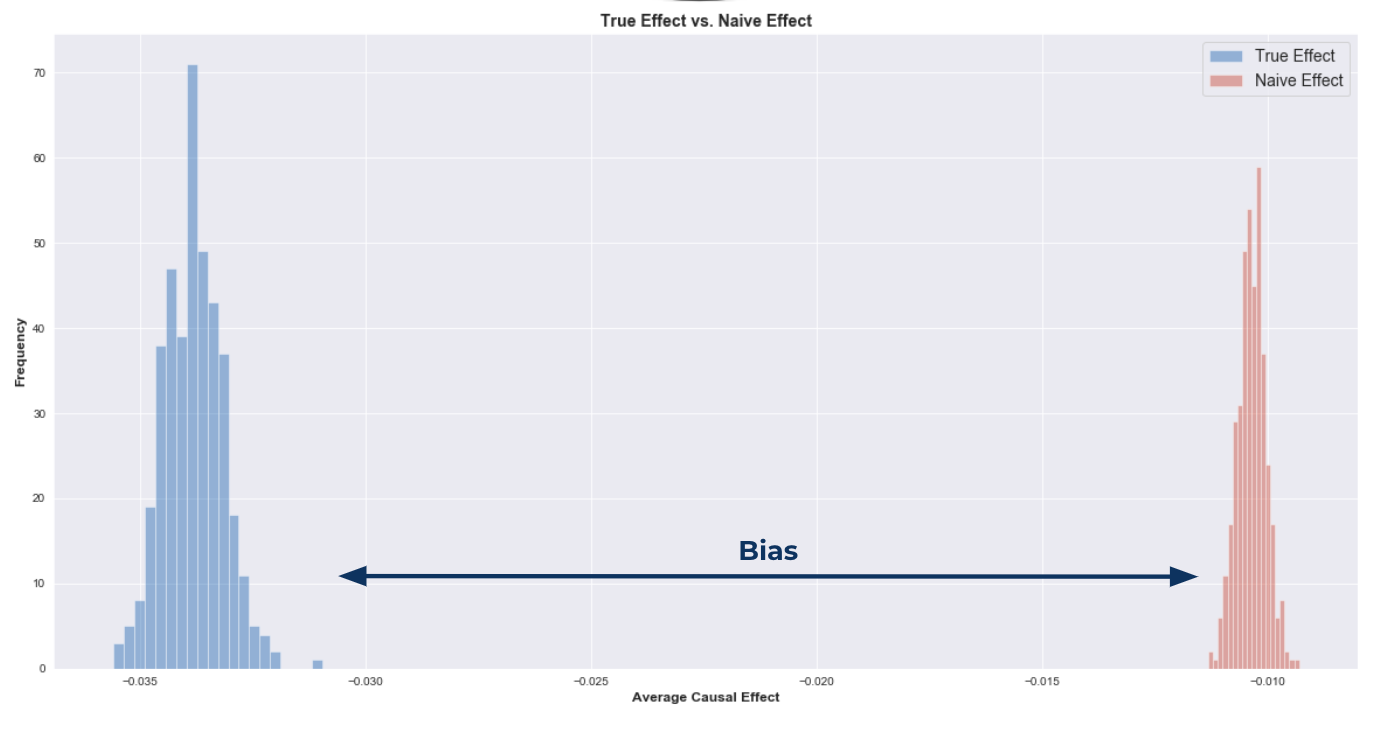
\includegraphics[width=0.95\textwidth]{histogram_selection_on_obs}
   \caption{Histograms of the probability of choosing Car Centric Modes under Different Data Generating processes.}
   \label{fig:histogram_probability}
\end{figure}

We have shown in this simulation exercise how causal graphs can be helpful in avoiding biased causal effect inferences.
Specifically, two situations highlight this fact; having mediating or confounding variables relative to the variable being intervened on in our outcome model.
In the case of mediating variables relative to the node the treatment intervenes on, we need to be careful about constructing our treatment effect estimator.
In particular, we need to ensure that we appropriately use total effect estimators instead of natural direct effect estimators.
Enacting a certain treatment shows its effect through the mediating variable.
Therefore, when ``changing'' the value of the intervention node, we need to make sure the values and distributions of any downstream nodes reflect this change.
For more information on mediating mechanisms, please refer to work by \citet{pearl_2012_mediation} and references therein.
In the case of confounding variables, we need to consider the treatment assignment mechanism when building choice models.
As \citep{hahn_2020_bayesian} show, one way to account for the treatment assignment mechanism is to estimate the propensity score in our sample and adjust for that in our outcome model.

In contrast to the example shown in this section, the data generating process might not be easily distinguishable in the majority of situations, mainly due to the complexity of the real world.
Therefore, constructing a causal graph that represents the data generating process as much as possible is not an easy task.
To prepare readers to create causal graphs, the next section will provide a brief overview of them and their history in choice modelling.
Then, Section \ref{sec:graph-construction} explores this topic and includes detailed guidance on how to build causal graphs representing the researchers beliefs about the data generating process.
Section \ref{sec:graph-testing} follows up with guidance on how to test one's causal graphs against one's data.


\section{Overview of Causal Graphs}

\subsection{Prior Uses of Causal Graphs in Choice Modelling}

With the introduction to causal graphical models given above, we (the authors) do not want readers to think that we believe the entire notion of a causal graph is foreign to choice modelling.
We do not think this is true.
We know that choice modellers have made use of causal graphs in various forms for years.
Here are two examples to illustrate our point.
First, consider the case of Random Utility Maximization (RUM) models.

For decades now, choice modellers have used stylized directed graphical models to denote or convey the meaning of their economic framework's notion of causality in the context of their research.
As an example, take the following figure from Walker and Ben-Akiva \cite authors.
In Figure \ref{figure_title} Walker and Ben-Akiva depict the assumption that covariates X cause random utilities U which collectively cause the choice via utility maximization.
The reason I call such diagrams stylized is because of their lack of detail of the relationships within the columns of the design matrix X.
When speaking of the covariates collectively, one is unable to distinguish whether one covariate causes another.
Such intra-covariate relationships are important for estimating the causal effects of a given policy, as demonstrated in Section \ref{Sec_label}.

Another area of relation with prior choice modelling literature is in Integrated Choice and Latent Variable (ICLV) models.
These models make inference on one or more latent variables, alongside the other parameters in one's model.
An example of such ICLV models is in Figure \ref{}, based on Figure \_bla\_ of Walker and Ben-Akiva \cite.
As with the causal diagrams for the RUM models, these causal diagrams are another set of graphical models that depict a certain set of structural modeling assumptions, a set of assumptions about the data generating process.


\section{(Initial) Causal Graph Construction}
\label{sec:graph-construction}

Construction of an initial causal graph typically proceeds as follows.
At a high level, we
\begin{enumerate}
   \item adopt a population perspective,
   \item brainstorm all variables that we think affect the system that generates our observations,
   \item remove any variables that could cause bias in our causal inferences,
   \item connect all variables in our graph according to our a-priori beliefs about causal relations amongst them
   \item consider how the graph structure may differ between individuals and subgroups within the population.
\end{enumerate}
The following paragraphs describe these steps in detail.

To begin, we adopt the position of a researcher concerned about population level relationships.
This means we will think through what is a likely generative model for all individuals.
Later in this section, we will devote time to thinking about how subgroups and individual heterogeneity may affect our causal graphs.

Now, we add our first variable(s) to our graph, the outcome variable(s) of interest in our problem.
Note that we should consider relations and dependencies between these outcomes, and we should draw these onto our graphs.
Such inter-outcome dependencies may be of great relevance or even focus.
Recall, for example, the case of activity-based modelers that was mentioned in Section \ref{sec:choice-graphs}.
Similarly, medical researchers with data on multiple health measures or companies with multiple business metrics may all be interested in how the outcomes cause each other.

After adding our outcomes to our graph, we list all the variables we believe to cause them.
We refer to these influencing variables as our initial explanatory variables.

Next, we iterate through these initial explanatory variables.
For each current explanatory variable in the iteration, we think of variables that may modify the effect of the current explanatory variable on the outcome(s) of interest.
We refer to these variables as effect modifiers\footnote{Note, effect modifiers and confounders are easily confused. Both variables cause the outcome. The difference is that effect modifiers do not cause the explanatory / treatment variables. Confounders do. For discussion and classification of the different types of effect modification, based on one's causal graph, see \citet{vanderweele_2007_four}}.
Note that some effect modifiers may be a part of our list of initial explanatory variables.
For any effect modifiers that we think of, outside of the list of initial explanatory variables, we add them to our causal graph.

Overall, modifiers are important because our treatment effects systematically vary with them.
Accordingly, if better understand when our treatments will be effective, then we can better target them.
% For instance, the effect of a transit voucher on increasing an individual's probability of using transit is likely modified by the recipients income.
% We expect a smaller treatment effect on wealthy individual's than on individual's with low income
For instance, imagine that a region-wide lockdown reduces the 14-day rolling average of new COVID-19 cases by X\% (on average).
Of course, we know that a lockdown's effectiveness is modified by the percentage of workers who must continue going out to work.
If most residents in an area are essential workers, then a lockdown will be less effective there, as compared with other locales.
We might wish to target other interventions for that region, as a replacement or supplement for the lockdown.
Targeting aside, knowledge of modifiers is also crucial to generalizing treatment effect inferences from one population to another.
To credibly transport our inferences, we must know what variables cause the treatment effects to differ between populations, and we must know how the distributions of those variables differs across populations \citep{pearl_2014_external}.

After adding explanatory and effect modifying variables to the graph, we turn our attention to mediating variables.
A mediating variable is one through which an explanatory variable influences our outcome(s) of interest.
Such variables have multiple uses.
Under certain instances of confounding, mediators enable the ``front-door'' criterion to identify one's causal effect \citep{glynn_2018_front, bellemare_2019_paper, gupta_2020_estimating}.
Similarly, subject to particular causal assumptions, mediating variables permit inference on long-term outcomes of a selected intervention, given only its short-term proxies \citep{athey_2019_estimating, yang_2020_targeting}.

To find these mediators, we again iterate through each explanatory variable.
On each iteration, we brainstorm variables along paths of influence from our explanatory variable to our outcome.
For instance, consider how the presence of a bike lane influences bicycle mode choice.
We hypothesize that an individual's subjective perception of safety is the primary (or sole) mediator through which bicycle lane presence influences mode choice.
Accordingly, we add subjective perception of safety to our causal graph for travel mode choice.

After considering the variables above, we turn our attention to variables that complicate our analyses.
To begin with, we think of confounding variables.
The process is similar to how we generated effect modifying variables.
We iterate through each of the explanatory, mediating, and effect modifying variables, thinking specifically of any variables that both cause the current variable in the iteration and cause the outcome variable(s).
We call these variables, which cause our outcome and current variables in the iteration, confounding variables \citep{elwert_2013_graphical, greenland_1999_confounding}.
As an example, consider a person's attitude towards environmental conservation.
This attitude may cause both that individual's observed distance to their workplace (another explanatory variable) and that individual's choice of travel mode.
Both in this example and in general, we should add such confounding variables to our causal graph.

Next, we consider the effects of selection.
As noted by \citet{greenland_2020_causal}, all datasets have a causal graph that implicitly conditions on a selection node.
I.e., we only analyze data that has been selected to be a part of our dataset.
We should therefore consider how all of the other nodes in our causal graph relate to the selection node.
In particular, will we suffer any selection bias due to the outcomes influencing whether an observation is selected for inclusion in our dataset?
Selection bias, if present, can cause our estimated causal effects to differ greatly from their population counterparts.
This stems from systematic differences between the observations that have been selected into our dataset and the observations in our population of interest.
For more details, see \citet{heckman_1979_sample} and \citet{hernan_2004_structural} as canonical references.

Another universally implied yet only implicitly described element of one's causal graph is the prior data and code that led to one's dataset \citep[Pg.7]{greenland_2020_causal}.
Presumably, prior data and potentially code-enabled-analysis influenced the sample design that led to your dataset.
Perhaps some data transformations and code to implement those transformations was used to convert a raw dataset into the dataset being used for causal inference.
And at all times, one uses computer programs to compute your reported results.
In each case, the prior data is variable that influences your current data, and your code is computational (sub)graph that is implicit in your causal graph.
These elements should perhaps be made explicit, and their influence on your causal effect estimates should definitely be assessed and reported.

Next, we should explicitly consider the role of time, even in research that may be cross-sectional due to the data that is available to us or due to the problem itself.
In reality, how do we think our system evolves over time?
If we consider multiple observations of a given decision maker, how does that decision maker's observed variables at time $t$ partially cause future variables important to the context or outcome(s) for that decision maker at time $t' > t$?
How do the actions of a decision maker $i$ at time $t$ partially cause the future context or outcomes of a decision maker $j$?
We should add explicit nodes to our graph, subscripted or denoted by time, to show the cross-time causal relationships in our system.
For in-depth discussion of time-related causal inference topics, see papers such as \citet{gill_2001_causal}, \citet{eichler_2007_granger}, and \citet{peters_2013_causal}.
Please note that the literature on this topic is vast, and the cited authors are not at all exhaustive or representative of all papers in this space.
Interested readers are encouraged to perform further literature searches on their own.

At this point, we have added to our causal graph all the outcome, explanatory, effect modifying, mediating, confounding, and time-indexed variables that we believe are relevant for our problem.
However, they are all disconnected nodes, i.e., singletons in the graph.
We now focus on pruning nodes from this graph, before drawing our final hypothesized connections.
In particular, we focus on pruning ``post-outcome'' variables that are not part of the causal graph for future time periods or other observations.
The reason for this is that conditioning on such post-outcome variables would bias our causal effect estimates.

To remove the problematic variables, we iterate through each of the non-outcome variables in our graph, and we assess whether each variable is actually a result of the outcome (perhaps in combination with other variables in our graph).
These post-outcome variables temporally follow the outcome variable(s) but do not cause variables in the causal graph for other observations.
We remove all such post-outcome variables from our graph.

Now is a good time to step back and consider what other researchers have thought about our problem.
Specifically, we should conduct a literature review to see how other researchers have conceptualized the topic that we are working on.
Have they included variables that we have not?
Were those variables related our outcomes of interest?
If so, should we add these variables to our causal graph? How should these variables enter our graph?
Do the included variables of other researchers suggest the existence of confounders in their work that we should include in our graph?
Have other researchers ascribed differing roles to our graph's current variables than we have?
For example, have other researchers judged a variable to be a confounder, when we solely thought of the variable as an effect modifier?
As we answer these questions, we should critically examine the evidence for these alternative decisions to see if we should also reconsider how we're judging our variables.

Finally, we need to connect the variables in our graph.
\begin{enumerate}
   \item Draw direct arrows from our explanatory variables, confounders, and effect modifiers to the outcomes.
   \item Draw arrows from the explanatory variables to the mediators, and then draw arrows from the mediators to the outcomes.
   \item Draw arrows from the confounders to the explanatory variables and mediators that they may cause.
   \item Draw arrows from the variables in time $t$ to the variables that they cause in time $t+1$.
\end{enumerate}
After drawing in all arrows, we should now have a fully connected causal graph.
Pause.
Take a moment to look over the graph to ensure there are no remaining singletons and that we have not drawn any spurious connections.
Then, take a moment to celebrate.
Drawing a project's first causal graph is hard work!

After celebrating, take a moment to pursue the following graph editing exercises.
First, think about how the graph might differ across sub-populations.
What sub-populations, if any, exist in your population of interest?
Are there any causal relationships that should, or should not, not exist for a given sub-population?
For instance, are the outcomes in some sub-populations independent of a given explanatory variable?
Can you think of any inverted causal relationships that are specific to this sub-population?
(I.e., for a given sub-population, does $B \rightarrow A$ instead of $A \rightarrow B$?)
Consider adding these sub-population indices to one's initial causal graph, or if this is not clear enough, draw modified causal graphs for each sub-population of interest.
Now, one can actually relax.
This concludes the ``purely mental'' drafting of one's causal graph.
In the next section, we'll look at testing this graph against data, and making any edits deemed empirically necessary.


\section{(Observable) Testing of Causal Graphs}
\label{sec:graph-testing}

\subsection{Description}
\label{sec:testing-description}
In the last section, we reviewed a process for creating an initial causal graph using expert opinion.
Critically, after drafting a causal graph, we should immediately test it against empirical data.
This is important because, if our graph captures inaccurate assumptions about the data generating process, then we have no reason to think that our conclusions from using the graph will be accurate.

To test our causal graphs against data, we will first test the implications of our graph that involve observable variables only.
We will defer the task of testing implications that involve unobserved / latent variables to the end  of this subsection.
For now, recall our discussion in Section \ref{sec:graph-overview} about the two basic implications of causal graphs: marginal independence and conditional independence.
In both cases, direct testing of marginal or conditional independence amongst nodes in the causal graph may be difficult.
Indeed, there are no direct tests of conditional independence that can detect all types of dependence, especially for continuous variables \citep{bergsma_2004_testing, shah_2020_hardness}.

As a result of this hardness, there are a myriad of research efforts aimed at testing conditional independence of two variables $X$ and $Y$, given a third variable $Z$ and any number of assumptions about the variables or the test statistic itself.
Some researchers proceed under the assumption that one has access to an approximation of the conditional distribution of $X \mid Z$ \citep{candes_2018_panning, berrett_2019_conditional}.
Other researchers designed conditional independence tests for general cases, assuming smoothness of the underlying data distributions and assuming accurate estimation of the distribution of the test statistic under the null hypothesis of conditional independence (e.g. \citet{zhang_2012_kernel, strobl_2019_approximate}).

Different from (but not excluding) these approaches, we will take an easier and less decisive route.
If a pair of variables have conditionally or marginally independent distributions, then their statistical moments will also be conditionally or marginally independent.
Instead of testing for marginal or conditional independence in distribution, we will perform a more tractable test for marginal or conditional independence in means.
If the variables in question are not conditionally or marginally independent in their means, then we know they are not independent in their distributions.
Conversely, even if a set of variables are marginally or conditionally independent in their means, this \textbf{does not} imply that the variables are independent in distribution.

This approach of indirectly assessing distributional independence by testing mean independence is not new.
The following papers have all proposed and implemented such an idea: \citet{burkart_2017_predictive, chalupka_2018_fast, inacio_2019_conditional}.
For conditional independences, the crux of the approach is to predict $Y$ based on $X$ and $Z$, then compare against a prediction of $Y$ based on a resampled value of $X$ and the original $Z$.
If $Y$ is mean-independent of $X$ given $Z$, i.e. $E \left[ Y \mid X, Z \right] = E\left[ Y \mid Z \right]$, then the predictive power of a model with resampled $X$ should resemble the predictive power of a model with the original $X$.
After all, in both cases, the conditional expectation of $Y$ is independent of one's $X$ values (real or resampled).
When assessing marginal independencies, one removes $Z$ from the models for the expectation of $Y$ and proceeds as described.

Note that as with the case of testing distributional independence, testing mean independence still requires researchers to make choices.
We have to select models for $E \left[ Y \mid X, Z \right]$ and $E\left[ Y \mid Z \right]$, respectively, for testing conditional and marginal mean-independence.
We also have to choose the performance statistic (e.g. $R^2$, log-likelihood, etc.) to compare these models.
Lastly, we also have to select a resampling method.
In particular, how (if at all) will our resampling strategy account for the possible dependence between $X$ and $Z$?

% State the choices made in this work.
% Provide some discussion of the alternatives and the effects of different choices.
For our demonstration, we made the following choices.
First, we used linear regressions to model $E \left[Y \mid X, Z \right]$ and $E \left[ Y \mid Z \right]$.
Second, we chose to use $R^2$ as our test statistic for judging the predictive performance.
Third, we have chosen to resample the $X$ vectors without replacement, keeping the length of the resampled vector equal to the length of the original vector.
In other words, we permute $X$.
And finally, we have chosen to visualize these tests by plotting a vertical line to display our observed test-statistic and by plotting the distribution of our test statistics based on the permutations of $Y$.

Our rationale for these choices are as follows.
In our dataset, most of our explanatory variables were continuous (at least in theory).
Accordingly, $R^2$ seemed a sensible performance metric for a model of the conditional expectation of a continuous random variable.

In contrast to our choice of performance metric, we chose our conditional expectation models and resampling methods based on empirical testing.
In particular, we created simulations to assess our mean-independence testing procedure.
We assessed the performance of our mean-independence testing procedures using simulations where $Y \leftarrow Z \rightarrow X$ and $X$ either did or did not cause $Y$.

Of particular importance were our simulations under the null hypothesis where $X$ was conditionally independent of $Y$.
Our initial simulations used random forests as our conditional expectation models and permutations as resampling methods.
Random forests are a non-parametric method that would allow us to have less fear of model misspecification, and permutations are easy to implement.
However, under the null hypothesis, we discovered that the tests based on the random forest models did not result in p-values that were uniformly distributed.
Given that we planned to use these procedures in a manner akin to hypothesis-testing, we hoped that our test statistics would be U-statistics.
When we switched from the combination of random forests and permutations to linear regressions and permutations, our p-values were indeed empirically, uniformly distributed.
Moreover, we still retained high power.

We do not claim that these choices for assessing mean independence will always be appropriate.
Indeed, one should assess one's tests on simulated data that resembles one's real data.
For our illustrative purposes though, the combination of linear regressions, permutations, and $R^2$ resulted in adequate tests of marginal and conditional mean-independence.

% Describe latent variable testing
Now that we have described testing with observable variables, we can more easily describe conditional independence tests that involve unobserved (i.e., latent) variables.
Indeed, when dealing with observational data, we will frequently find ourselves not having observed all variables that are of interest.
Nevertheless, we still wish to test whether our data contradicts our graph.
One way to directly extend our conditional independence testing to account for latent variables is to adopt a missing data perspective and impute the latent variables from a prior distribution.
In particular, we can generalize our previous tests as follows.

First, we can consider that instead of performing one test with a set of observed $X$, observed $Y$ and observed $Z$, we instead perform tests of observed $X$, observed $Y$, and imputed $Z$.
This recasts the randomness underlying the null-distribution in our original test statistic of $R^2$ as a function of our permutation of $Y$ and our imputation of $Z$.
Here, we impute $Z$ by sampling from the prior or posterior distribution of $Z$, depending on whether we're testing independencies before or after performing inference on our model's parameters.
Moreover, we'll now compute the p-value of this test statistic by marginalizing over the permutations and imputations.
Specifically, our p-value will be $\mathcal{E}_{\textrm{samples, permutations}} \left[ 1_{R^2 \left( X, Y, Z_{\textrm{sampled}} \right) <  R^2 \left( X_{\textrm{sampled}}, Y_{\textrm{sampled, permuted}}, Z_{\textrm{sampled}} \right)} \right]$.
For reference, this is the same as the p-value for test statistics (or discrepancies) defined in \citet[Eq. 7]{gelman_1996_posterior}.

Lastly, because our test statistic is itself a random variable that depends on the imputed values of $Z$, we must change our visualization method.
Instead of plotting a single line versus a distribution, we now plot two distributions against one another.
We first plot the distribution of ``observed'' test statistics that is computed using the observed $X$, observed $Y$ and imputed $Z$ values.
Then, we plot the distribution of ``sampled'' test statistics using prior samples of $\left( X, Y, Z \right)$ as a reference.
For an example of such a plot, see Figure \ref{} (discussed in the following subsection).
Note, we have one value per imputed vector $Z$ in both the observed and sampled distributions.
However, for the distribution of ``sampled'' test statistics, we marginalize over permutations of $Y$ since this distribution represents the null hypothesis of conditional or marginal independence.

Of course, since there is generally ``no free lunch,'' this approach comes with drawbacks.
One major concern is that such tests are very sensitive to assumptions about the joint prior distribution, $P_{\textrm{prior}} \left( X, Y, Z \right)$
In our experience using simulation, if the observed data $\left( X, Y \right)$ is unlikely under the joint prior distribution $P_{\textrm{prior}} \left( X, Y, Z \right)$ then the conditional independence test is likely to fail.
As always, the failing test indicates that the observed data is unlike the data simulated and used to construct the reference distribution.
However, in this case, the dissimilarity may not relate to the conditional independence properties but may instead be an artifact of the sampled $\left( X, Y \right)$ being generally dissimilar to the observed $\left( X, Y \right)$.
This highlights the need for extensive prior predictive checking of one's assumed joint prior, $P_{\textrm{prior}} \left( X, Y, Z \right)$, \textit{before} using conditional independence tests on causal graphs with latent variables.

\subsection{Demonstration}
\label{sec:testing-demonstration}

% Illustrative causal graph
To demonstrate the testing procedures described above, we used the causal graph in Figure \ref{fig:graph-for-testing}.
This causal graph shows a set of hypothesized causal relationships between variables thought to contribute to the utility of the drive-alone travel alternative in our dataset.
As drawn, this graph encodes multiple marginal and conditional independence assumptions.
Tools such as Daggity \citep{textor_2016_robust} can be used to automatically infer all independencies based on one's graph.
For didactic purposes, however, we focused our attention on two particular independence assumptions.

First, we tested the assumption of marginal independence between the number of licensed drivers and the number of automobiles in a household.
A-priori, we may expect this independence to be have low-probability since the number of automobiles may generally be positively related to the number of licensed drivers in a household.
Secondly, we tested the assumption of that travel cost was independent of travel time, conditional on travel distance.
Unlike the first independence that we focus on, this conditional independence assumption is a-priori more credible.
Despite their differing levels of a-priori credibility, we will see how we can test both using the procedures described in the previous subsection.

% Marginal testing results
% \begin{figure}
% \centering
% \includegraphics[width=0.5\textwidth]{exa}
% \caption{Example decision tree for bicycle consideration}
% \label{fig:marginal-independence-test}
% \end{figure}

In particular, Figure \ref{fig:marginal-independence-test} shows the results of using permutation, linear regression, and $R^2$ to test the hypothesis of marginal independence between the number of automobiles and the number of licensed drivers in a household.
The empirical p-value of 0 confirms that the observed data is unlikely given the null-hypothesis of marginal, mean-independence.
More specifically, when regressing the number of licensed drivers in a household on the number of cars in that household, one achieves an $R^2$ near 0.4.
In contrast, when permuting the number of cars in the household and re-estimating the regression, the distribution of p-values concentrates around 0.
This plot visualizes the fact that---through the lens of our chosen test statistic ($R^2$), linear regression model, and permutation-based resampling strategy---data generated under an assumption of marginal mean-independence does not ``look like'' the observed data.
Accordingly, we should consider the weaker assumption of marginal dependence, where we can make data-generating assumptions that offer greater realism and concordance with our observations.

% Conditional testing results
% \begin{figure}
% \centering
% \includegraphics[width=0.5\textwidth]{exa}
% \caption{Example decision tree for bicycle consideration}
% \label{fig:conditional-independence-test}
% \end{figure}
In Figure \ref{fig:conditional-independence-test}, we have an analogous visualization of a conditional independence test.
Here, we test the hypothesis that travel time is mean-independent of travel cost, conditional on travel distance.
To execute this test, we model the conditional expectation of travel time as a linear function of travel cost and travel distance.
As with the marginal independence test results, the $R^2$ of the model using the observed values of travel cost are greater than the model's $R^2$ using any simulated datasets.
Again, this means that the $R^2$ using observed data is unlikely given our method of sampling from the null distribution of $R^2$ given conditional, mean-independence of travel time and travel cost.

As before, we should respond to this result by considering conditional dependence between our variables of interest.
In particular, we should investigate the idea that travel time is associated with travel cost, conditional on travel distance.
Why might this be the case?
Does travel time cause travel cost when driving alone?
Does travel cost cause travel time while driving alone?
Does some other set of variables (potentially unmeasured) cause both travel time and travel cost?

Thinking through these questions, we can immediately think of latent variables that cause both travel time, travel cost, and the choice.
For example, consider whether one drives alone over the San Francisco Bay Bridge.
If one crosses the bridge, then traffic delays will likely increase one's travel time.
Moreover, if one crosses the bridge, then one's travel cost is higher due to tolls that one must pay.
And finally, if one takes a toll lane to get across the bridge faster, then one also pays a higher price.
Overall, we can think of intuitive explanations for why there might be a dependence between travel time and travel cost, even after conditioning on travel distance.
These explanations suggest particular relationships to analyze and particular variables, such as bay bridge crossings, to include in one's mode choice (i.e. outcome) model.

\subsection{Additional techniques}
\label{sec:testing-addendum}

The methods presented in this section have focused on testing independence assertions using one's dataset.
While this approach may be the most accessible strategy for testing one's causal graph, there are other applicable techniques.
For instance, \citet{pitchforth_2013_proposed} put forth a detailed checklist of qualitative questions for one's causal graph.
Answering these questions should increase the trustworthiness of one's graph.
Alternatively, there are other quantitative tests of one's causal graph that were not explored in this section.

For instance, a causal graph makes assumptions about the number of independent variables in one's dataset: i.e., the nodes in one's graph without parent-nodes.
One can test this assumption by estimating the ``intrinsic dimension'' of one's data, and testing whether the intrinsic dimension equals the number of independent variables implied by one's graph.
For more information on estimating the intrinsic dimension of a dataset, see \citet{camastra_2016_intrinsic, song_2019_identification}.
See \citet{chenwei_2019_likelihood} for an extension of this idea for the situation where one suspects or cannot rule out unobserved confounding.

% Test vanishing tetrads / t-separation
Another empirical implication of one's causal graph is the existence of so-called ``vanishing tetrads'' \citep{spearman_1904_general}.
This term signifies that the difference between the product of two particular pairs of covariances must be zero.
As stated, this implication of one's causal graph is hard to intuitively understand.
However, one can graphically determine the existence of vanishing tetrads and determine which variables are part of these tetrads.
Once one has determined the tetrads that should vanish according to one's graph, one can estimate the corresponding covariances and test to see if their difference of products is indeed unlikely to be zero.
Such a test is yet another way to empirically determine whether one's graph is incompatible with one's dataset.
For the original theorems proving that tetrads can be graphically identified and characterized, see \citet{shafer_1996_vanishing} and references therein.
For a more detailed and intuitive explanation of the graphical criterion for vanishing tetrads, see \citet{thoemmes_2018_local}.

% Test functional inequalities / constraints, i.e. entropy constraints / inflation technique
Finally, we note that there are still a whole host of other techniques for testing one's causal graphs.
Many of these remaining techniques are useful when one's causal graph contains unobserved (i.e., latent) variables.
On one hand, we can use ``triad constraint'' tests that test independence between ``pseudo-residual'' values and one's explanatory variables \citep{cai_2019_triad}.
Results from these tests are particularly useful for judging assumptions about how unobserved variables in our graph relate to each other and to our observed variables.

Relatedly, one can make use of constraints on entropies of our observed variables instead of independencies.
The basic idea is that differing assumptions about the structure of the unobserved variables in our graph imply differing amounts of entropy in the variables that we do observe, so we should test for these differences in entropy.
For more information and examples, see the literature about:
\begin{itemize}
  \item inequality constraints, e.g. \citet{tian_2002_testable, kang_2006_inequality, ver_2011_sequence}
  \item information inequalities, e.g. \citet{chaves_2014_inferring}
  \item entropic inequalities, e.g. \citet{chaves_2014_causal}
  \item the inflation technique, e.g. \citet{wolfe_2019_inflation, navascues_2020_inflation}
\end{itemize}


\section{Causal Discovery}
\label{sec:causal-discovery}

% How is causal discovery related to testing causal graphs?
In the previous section, we detailed one method for testing the marginal and conditional independence assumptions of one's causal graph.
As presented, this strategy requires one to first have a causal graph.
Indeed, this requirement is why Section \ref{sec:graph-construction} provides instruction on how to construct an initial causal graph using expert opinion.

The unstated presumption is that one will test one's working causal graph, and if any of tests fail, one will then revise the graph until all assumptions appear plausible.
Essentially, one proceeds in a loop of postulating, testing, and editing one's causal graph until it is not blatantly contradicted by one's data.
If this sounds tedious, one can consider making one's computer work for you.
Specifically, by exchanging the human-in-the-loop for a purely algorithmic endeavor, one arrives at the practice of  causal discovery: inferring one's causal graph from one's data.

This section will describe why causal discovery is important, provide a brief overview of the main concepts in causal discover, and show the results of using causal discovery algorithms on the dataset described in Section \ref{sec:graph-importance}.

\subsection{Why use causal discovery?}

% Why is causal discovery important?
% Promotes robustness and understanding of results
% Inspires creation and editing of expert-opinion graph
% Aids characterization of posterior uncertainty
As a topic of study, causal discovery is important for numerous reasons.
Three of these reasons are the following.
First, causal discovery promotes robustness and understanding of our causal effect estimates.
By comparing against our causal effect estimates when using a data-driven causal graph, we can begin to understand how our prior beliefs affect our estimates.
Secondly, causal discovery helps inspire creation and editing of expert-opinion graphs.
Indeed, it's typically easier to edit than to create from scratch.
Graphs found via causal discovery can spark ideas for one's own graph if they feature different causal relations than are present in one's own graph, and they provide a starting point for graph revision.
Thirdly, causal discovery algorithms can aid characterization of posterior uncertainty in one's causal graph and causal effect estimates.
Each causal graph discovered from one's data represents an alternative way of understanding the world, and we can quantify the probability of each of these causal models representing our data generating process.

% Why does causal discovery help robustness and model understanding?
Let's begin with robustness.
Here, one way of reducing the probability of incorrect inferences is to give oneself multiple chances to be correct.
In particular, the Section \ref{sec:graph-testing} tested, expert-opinion based graph was never meant to be the stopping point in one's exploration of possible causal relationships.
Instead, we advocate using multiple graphs to help us understand our causal effect estimates.

Specifically, consider that a causal graph is equivalent to a square matrix with one row for each variable, and binary entries that denote whether the variable for the row causes the variable on the column \citep[p. 3]{glymour_2019_review}.
A prior that expresses maximum ignorance over the graphs would be a prior where each matrix entry followed its own Bernoulli distribution with $p=0.5$.
Conversely, a prior expressing maximum certainty over the graph could be a prior with 100\% certainty that our expert-opinion graph is the true causal graph.
These two extremes represent reference priors that we can use in sensitivity analyses.
By observing the distribution of causal effect estimates under each prior, we can reflect the uncertainty from not knowing the ``true'' causal graph, and we can begin to understand the ways that our estimates are sensitive our prior beliefs.

% How does causal discovery help inspire our creation and editing of an expert-opinion causal graph?
Beyond increasing our understanding of our estimates, causal discovery algorithms can help us create causal graphs based on expert-opinion.
In particular, criticizing causal graphs is easy.

As noted by \citet[p. 708]{pearl_1995_causal}, ``every pair of nodes in the graph waves its own warning flag in front of the modeller's eyes: `Have you neglected an arrow or a dashed arc?''
Additionally, the presence of directed causal relations is vividly placed before one's eyes for immediate criticism (e.g., is $X \rightarrow Y$ plausible?).
Similarly, undirected or bi-directed edges between variables highlight causal ambiguity, thereby inviting analysts to resolve the question of directionality in the relationship.
And conversely, we may learn from causal links (i.e. arrows) that are present in the graphs output from our causal discovery algorithm that we initially overlooked.
By contrasting and criticizing alternative graphs, we clarify the strengths and deficiencies of our own point of view.
Then, once we've identified elements that we think should or should not be present in a causal graph for our dataset, we can amend our hand-crafted graph to meet these requirements.

% How does causal discovery help characterize posterior uncertainty about the  true causal graph?
% Weighted bootstrap posterior
Lastly, causal discovery can help us characterize our posterior uncertainty about the data-generating causal graph.
They enable approximation of the posterior distribution over causal graphs, in at least two ways.
One approach is to use a weighted likelihood bootstrap approximation \citep{newton_1994_approximate} to the posterior distribution over graphs.
In this approach, one would first sample a vector of weights for the likelihood terms.
Then, one would use those weights in one's causal discovery algorithm to produce a single `sample' from the posterior approximation.

%Randomize-then-optimize.
Alternatively, we could use yet another randomize-then-optimize \citep{bardsley_2014_randomize, orabona_2014_measure} approach to sampling from an approximate posterior distribution.
Here, one would sample from a prior on entries of the matrix representation of a causal graph.
Semantically, we sample constraints such as ``$X \rightarrow Y$ (MUST | MUST NOT) be in the causal graph''.
We ``sample'' from the approximate posterior by running the causal discovery algorithm on the original dataset, with the inclusion of these randomly generated constraints.
And, of course, we can consider hybrids of these two posterior approximation schemes.

With these posterior approximation methods, we can generate causal graphs for all the purposes mentioned above:
\begin{itemize}
   \item for criticism and inspiration,
   \item for distributional analyses of one's causal effect estimates conditional on each sampled graph, and
   \item for distributional analyses of the causal graphs themselves.
   \newline
   I.e., how certain are we of any one causal graph?
\end{itemize}

\subsection{Overview of causal discovery algorithms}

% Pointers to thorough review papers
The following subsection presents a non-exhaustive overview of causal discovery algorithms.
For conciseness, an exhaustive review of causal discovery algorithms is out of the scope of the article.
Crucially, we rely heavily on review papers such as \citet{glymour_2019_review} and \citet{spirtes_2016_causal} to fill in our gaps.


% Types of causal discovery algorithms
Overall, there are three classes of causal discovery algorithms.
One class attempts to directly infer the marginal and conditional independences in one's causal system.
That is, this class of algorithms identifies a so-called Markov Equivalence Class (MEC) of graphs.
Considering the discussion of independence testing in Section \ref{sec:graph-testing}, this class of algorithms is perhaps best understood as repeated and systematic independence tests.
These causal discovery algorithms are constraint-based algorithms, because the observed independencies represent constraints that define the space of plausible causal graphs for the dataset.
Common constraint-based algorithms include the Peter-Clarke (PC) algorithm and the Fast Causal Inference (FCI) algorithm \citep{glymour_2001_causation}.
The PC algorithm assumes no unobserved confounding variables, whereas the FCI allows for (and sometimes infers) the presence of such unobserved confounders.

% DESCRIBE SCORE BASED DISCOVERY ALGORITHMS
The second class of algorithms are known as score-based algorithms.
They proceed sequentially by pairs of variables, making changes with a constraint on how their chosen score is affected by this change.
First, we start from a fully disconnected graph, and we add directed causal relationships so as to increase the score of the generative model that corresponds to our graph.
Then, once we have found the graph structure that maximizes the score on our data, we prune as many directed causal relationships as can be done without harming our score.
In the end, the algorithms return the resulting set of graphs that retain maximal score.
Common score-based algorithms include the Greedy Equivalence Search (GES) algorithm \citep{chickering_2002_optimal}.
Typically these methods operate under stricter assumptions than constrain-based methods, but combinations of the two ideas have often outperformed methods that are strictly in either class \citep{glymour_2019_review}.

% DESCRIBE FCM ALGORITHMS
Lastly, the third class of algorithms relies on hypothesized Functional Causal Models (FCM) \citep{goudet_2018_learning} for each of the variables in one's system, as a function of their parents.
The defining characteristic in such algorithms is that they exploit asymmetries in the residuals of models for the hypothesized relationships of $X \rightarrow Y$, $Y \rightarrow X$.
In particular, the residuals will be independent of the hypothesized cause in only one of the two potential models.
As noted in the description of such algorithms, they are especially useful for discovering causal relationships between pairs of variables.
In other words, discovery methods based on FCMs enable orientation of the undirected or bi-directed edges that represent ambiguity over whether $X \rightarrow Y$ or $Y \rightarrow X$.
This orienting capability can be usefully combined with the previous causal discovery algorithms that infer classes graphs with equivalent marginal and conditional independencies.
And of course, extensions of these techniques exist for inference in the presence of unobserved confounding \citep[Sec. 6]{goudet_2018_learning} and for learning an entire causal graph as opposed to only dealing with variable pairs \citep{zheng_2020_learning}.

% What questions can be addressed via these discovery algorithms
% $X \rightarrow Y$ or $X \leftarrow Y$
% Full graph inference (with and without allowance-for / detection-of latent confounders)
% Discovery of equivalence classes

\subsection{An application of causal discovery}


\section{Introduction}
\label{sec:intro}

The following chapter is concerned with the existing disconnect between the 
fields of travel demand modeling and causal inference. 
More specifically, the chapter is motivated by the current lack of use of methods and findings from 
the causal inference literature in travel demand modeling. 

More often than not, the development of behavioral models in transportation, 
specifically transportation demand models, is driven by the need to evaluate 
the impact of external interventions, in the form of alternative policies, on a 
certain outcome of interest. 
These questions that transportation demand models 
are built to answer are causal by definition: we are interested in how the 
system reacts to \textit{external} interventions. 
Yet, when those models are 
developed, there is very little consideration given to causality, and when 
causal concepts are accounted for, the process is done implicitly without a 
formal framework. 

While the field of transportation demand modeling could benefit greatly from 
incorporating causal inference techniques, there are barriers that have made 
this integration slower than what one would hope. 
These barriers stem from the difference between the types of problems transportation demand modelers deal with and those that are typically studied in the causal inference literature. 
Perhaps the main fundemental difference is that demand modelers 
are typically trying to forecast the impacts of policies that haven't been 
implemented or seen before, which requires additional work and a change to the
typical causal modeling workflow in order to translate a given policy 
(treatment) into a set of characteristics and variables that exist in the
data and system at hand (please refer to \citet{brathwaite_2018_causal} for a 
more thorough discussion of those barriers). 
While those barriers make the problem of demand modelers harder, there is still a lot to gain from 
incorporating causal inference techniques where appropriate, and to contribute
in turn where the literature lacks.  

The relevance of this topic now is motivated by the significant boost in the causal inference literature recently, both in the potential outcomes and the causal graphical modeling frameworks.
The goal of this chapter is to formalize a workflow for approaching 
transportation demand modeling problems from a causal perspective. 
We will draw heavily on the use of directed acyclic graphs (DAGs) formalized by \citet{pearl_causality_2000} as a means of representing the modeler's knowledge and assumptions about a given problem. 
The chapter will provide an overview of DAGs, the 
testable implications that come with one's causal representation, the main 
tests that one could do to falsify or justify a given causal graph, and then how 
to use a causal graph to estimate the causal relationships of interest. 
We will demonstrate the use of this framework through simulations, where we 
clearly show the benefits and implications of this approach as opposed to 
traditional approaches. 
The last part of this chapter deals with the more complicated issue of latent 
confounding, where one variable confounds two or more variables in the causal 
graph. This type of confounding creates variations in the outcome variable that are not caused by 
the confounded variables but are correlated with it, which biases the estimated 
causal effects of those variables if nothing is done to account for the 
confounding. 
We focus on a recent technique to deal with latent confounding suggested by \citet{wang_2019_blessings} to address unobserved confounding when collecting additional data is not feasible. 
We describe this problem in more details in section 7.


\section{Conclusion}
\label{sec:conclusion}

Travel demand problems aim at forecasting the impact of proposed project and policies. These problems are causal in nature. 
To our surprise, there has been very little mention of causal inference in the field of travel demand modeling.
\citet{brathwaite_2018_causal} have documented this disconnect and presented an initial framework for addressing it.

In this chapter, we build up on \citet{brathwaite_2018_causal} and highlight the importance of using causal graphs and 
causal inference methods in transportation demand modeling efforts.

We presented a numerical exercise aiming to show the importance of  the data generating process in the estimation 
of effects of interest resulting from external interventions. 
We showed, using the same outcome model, that different assumptions about the data generating processes could 
lead to bias in estimates of the effect of interest.

Data generating processes can be illustrated effectively using DAGs as shown by \citet{pearl_1995_causal}.
We have shown that DAGs help researchers and practitioners represent their assumptions about the data generating process. 

We presented a process allowing researchers and practitioners to construct causal graphs based on their expert opinion of the problem at hand. 
We also presented methods for testing the implications encoded in the the practitioners proposed causal graph. 
These implications might be either observed, latent, or both.

Beyond testing the implications and assumptions encoded in a one's causal graph, we describe why causal discovery is important in discerning relationships between covariates one's data.
We shortly presented several causal discovery algorithms used by
other researchers in different fields. 
We highlighted the use of one of these causal discovery algorithms on a simple example. 
We showed that causal discovery methods help us test independence within our data, 
develop a clearer picture about the uncertainty within the variables shown in the causal graph, 
and expand the level and amount of tests performed on our data when compared to the tests implicated 
by the structure of the researcher's proposed causal graph.

We presented examples of latent confounding within the transportation demand modeling field and highlight 
some examples of current methods aiming at addressing problems resulting from confounding in certain situations.

We present a recently developed algorithm by \citet{wang_2019_blessings} aiming to address the problems not 
addressed by previously developed methods dealing with confounding. We use this model on the same example illustrated in
the selection on observables simulations and highlight the instances where it leads to a better recovery of 
a confounder in one's causal graph. 

We then show that while the deconfounder algorithm might be a promising step in the right direction, 
it still has some notable deficiencies. More specifically, we show that the deconfounder algorithm shows 
to be sensitive to small errors in one's data.


\bibliography{main}

\end{document}




